\documentclass{article}

\usepackage{listings}
\usepackage[english]{babel}
\usepackage{color}
\usepackage{graphicx}
\graphicspath{{img/}}

\interlinepenalty 10000

\definecolor{dkgreen}{rgb}{0,0.6,0}
\definecolor{gray}{rgb}{0.5,0.5,0.5}
\definecolor{mauve}{rgb}{0.58,0,0.82}

\lstset{frame=tb,
  language=C++,
  aboveskip=3mm,
  belowskip=3mm,
  showstringspaces=false,
  columns=flexible,
  basicstyle={\small\ttfamily},
  numbers=none,
  numberstyle=\tiny\color{gray},
  keywordstyle=\color{blue},
  commentstyle=\color{dkgreen},
  stringstyle=\color{mauve},
  breaklines=true,
  breakatwhitespace=true,
  tabsize=3
}

\title{Spyke (Babel Project)}
\author{La Pintade}
\date{5 Octobre 2015 - 8 Novembre 2015}

\begin{document}

  \maketitle
  \tableofcontents


  \newpage
  \section{CLIENT}
  \subsection{GUI}
    \begin{lstlisting}
  class PTUser
  {
    private:
      class User
      {
        std::string _username;
        std::string _password;
        std::string _objectId;
        std::list<Contact*> _contactList;
      public:
        User();
        ~User();
        const std::string &getUsername() const;// Get the username of the current user
        const std::string &getPassword() const; // Get the password of the current user
        const std::string &getObjectId() const; // Get the objectId of the current user
        void setUsername(); // Set the username of a new user
        void setPassword(); // Set the password of a new user
        void setObjectId(); .// Set the object ID gotten from the server
        std::list<Contact*> getContactList() const; // Return the contact list of the current user
        const std::string &getLocation() const; // Return the location info of the current user
        void addContact(Contact&); // Add a new contact to the contact list of the current user
      };
      User	_currentUser;
      NetworkServerHandler server;
      std::string _ipServer;
    public:
      PTUser();
      ~PTUser();
      User&		currentUser();
      template<typename T>
      void signUp(T &obj, void(T::*call)(int), const std::string &username, const std::string &password, const std::string &i);
      void logUser(T &obj, void(T::*call)(int), const std::string &username, const std::string &password, const std::string &ip);
        // The function logUser will call the server to check if the user exist, if not it will call the callback function with an error value set to 1, else it will call with an error value set to 0.
      }
  };
      extern PTUser g_PTUser;
\end{lstlisting}

\newpage

\subsection{NETWORK}

\begin{lstlisting}

  class NetworkServerHandler : public QObject
  {
    Q_OBJECT
  private:
    QObject *parent;
    QTcpSocket *_socket;
    std::string _host;
    unsigned int _port;
  public:
    NetworkServerHandler(QObject *parent = 0);
    ~NetworkServerHandler();
    int start(const std::string &host, unsigned int port); // Launch the connection between server and client /\ Return -1 if failed, 0 if success.
    void setHost(const std::string &); // Set the host of the server
    void setPort(unsigned int); // Set the port of the server
    const std::string &readSocket(); // Read data from server
    void writeSocker(const std::string&); // Write data on server
  private slots:
    void	readyRead(); // Callback function from QT /\
    void	connected(); // Callback function from QT /\ Is called when connection has succeed
  };

\end{lstlisting}
\newpage
\subsection{Network Client Handler}
\subsection{Audio Encoder}
\subsection{Audio Handler}
\subsection{Thread}
\subsection{Contact}
\newpage
\section{SERVER}

\subsection{LoginWidget}
  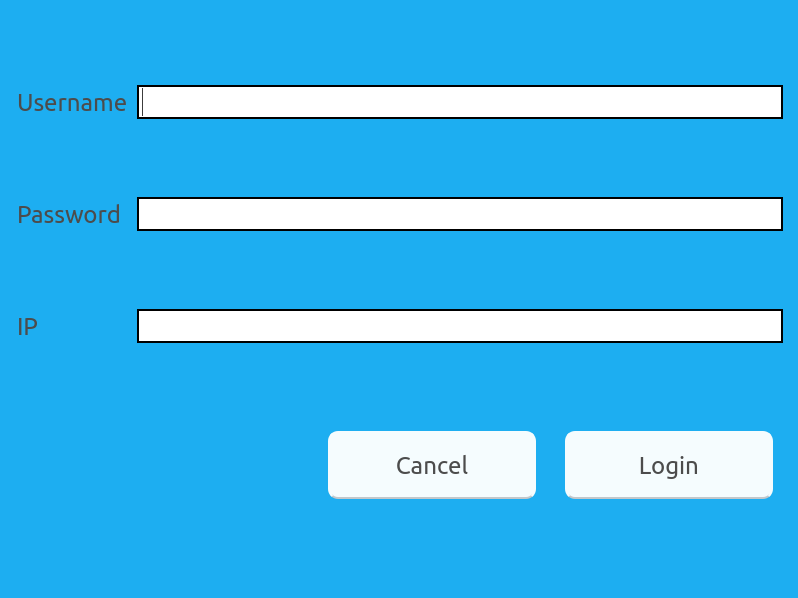
\includegraphics[width=350]{LoginWidget}
  \newpage
\subsection{MainWidget}
  
\includegraphics[width=350]{TabsBabel}
  \newpage
\subsection{SignupWidget}
\subsection{Home}
\subsection{Contact}
\subsection{Conversation}
  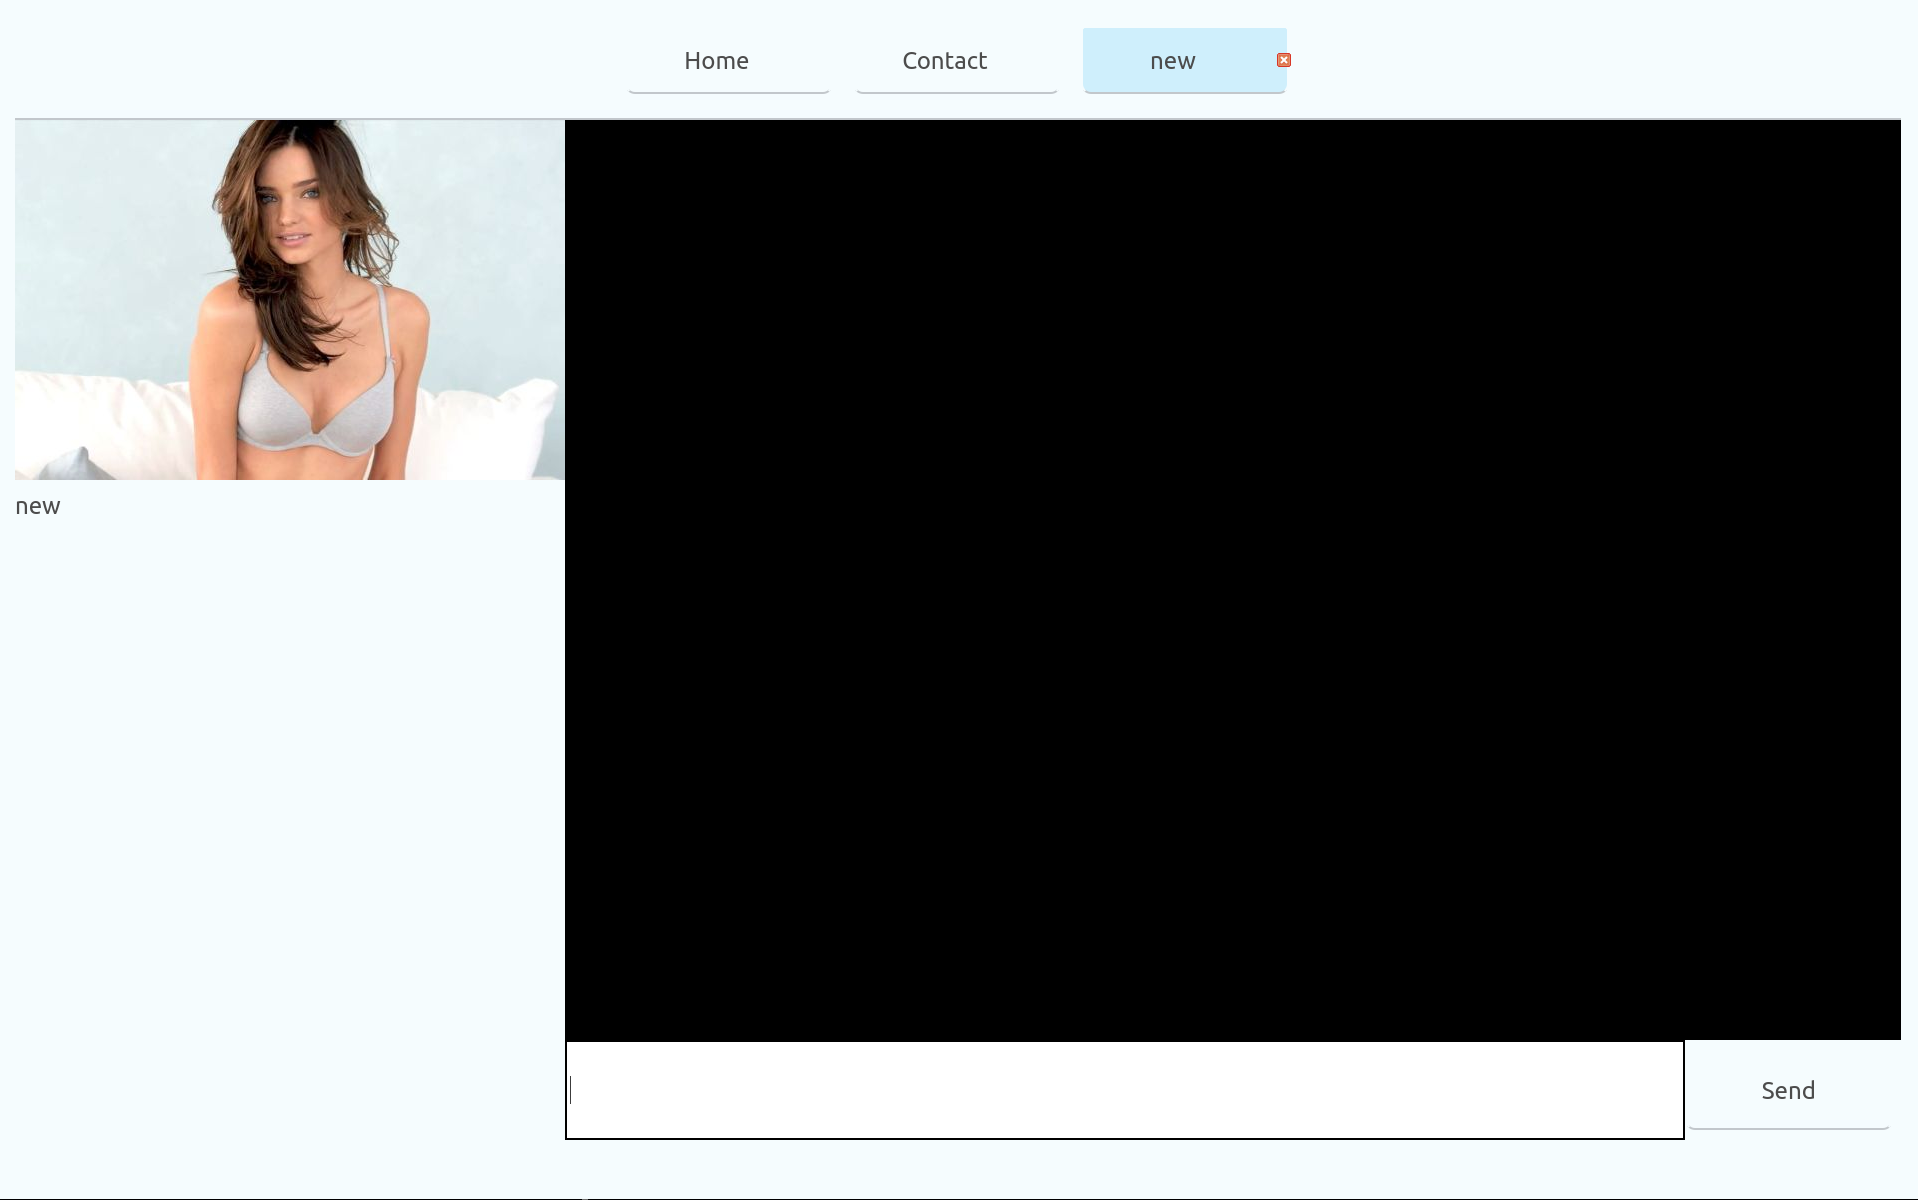
\includegraphics[width=350]{ConversationWidget}
\subsection{Notifications}

\end{document}
